\documentclass[11pt]{report}
\newcommand{\sizetwelvefixed}{\fontsize{11}{11}\selectfont}
\usepackage[top=25mm, bottom=20mm, left=40mm,right=25mm]{geometry}
%%\usepackage[margin=1in]{geometry}
\usepackage{mathptmx}
%%\usepackage[scaled=.90]{helvet}
\usepackage{times}
\usepackage{lipsum}% just to generate filler text
\usepackage{setspace}
\doublespacing
\usepackage{graphicx} % support the \includegraphics command and options
\usepackage{titlesec}

%%%%%%%%%%%%%%%%%



%For inserting Python Code
\usepackage{listings}
\usepackage{color}
\definecolor{dkgreen}{rgb}{0,0,0}
\definecolor{gray}{rgb}{0,0,0}
\definecolor{mauve}{rgb}{0,0,0}
\lstset{ %
language=Python, % the language of the code
basicstyle=\footnotesize, % the size of the fonts that are used for the code
numbers=left, % where to put the line-numbers
numberstyle=\tiny\color{gray}, % the style that is used for the line-numbers
stepnumber=1, % each line is numbered
numbersep=12pt, % how far the line-numbers are from the code
backgroundcolor=\color{white}, % choose the background color. You must add \usepackage{color}
showspaces=false, % show spaces adding particular underscores
showstringspaces=false, % underline spaces within strings
showtabs=false, % show tabs within strings adding particular underscores
frame=single, % adds a frame around the code
rulecolor=\color{black}, % if not set, the frame-color may be changed on line-breaks within not-black text (e.g. commens (green here))
tabsize=2, % sets default tabsize to 2 spaces
captionpos=b, % sets the caption-position to bottom
breaklines=true, % sets automatic line breaking
breakatwhitespace=false, % sets if automatic breaks should only happen at whitespace
title=\lstname, % show the filename of files included with \lstinputlisting;
% also try caption instead of title
keywordstyle=\color{dkgreen}, % keyword style
commentstyle=\color{dkgreen}, % comment style
stringstyle=\color{dkgreen}, % string literal style
escapeinside={\%*}{*)}, % if you want to add a comment within your code
morekeywords={*,...} % if you want to add more keywords to the set
}

%%%%For inserting Python Code Ove



%%%%%%%%%%%%%%%%%







\begin{document}
\setlength{\headsep}{4pt}
\newpage
\renewcommand{\baselinestretch}{1.2}\normalsize
%Renames "Bibliography" to "References" on ref page


\renewcommand\bibname{References} 
\begin{document}
\begin{center}
\thispagestyle{empty}
\vspace*{1\baselineskip}

\large{\textbf{Thought Cloud Treasure Hunt Android Game}}\\[1.0cm]
\large{\textbf{ABSTRACT}}\\[0.5cm]
\end{center}
\thispagestyle{empty}
\large{\emph{}

Thought Cloud  is a social thinking platform that intends to bring people together by the way they think. The concept came into picture by a thought about connecting people who are thinking about the exact same thing at the same time.\\ Thought Cloud relies its core strength on -Preciseness - Restricted to three words long thoughts only.Lucidity - Easy and interactive design makes it a child's play to use it. Innovation - Innovative feature of real time thought mapping by demography. Thought Cloud c:geo is a simple to use but powerful geocaching client with a lot of additional features. All you need to get started is an account on geocaching.com. Find caches using the live map or by using one of the many search functions. Navigate to a cache or a waypoint of a cache with the built-in compass function, the map or hand over the coordinates to various external apps (e.g. Radar, Google Navigation, StreetView, Locus, Navigon, Sygic and many more 

Store cache information to your device directly from geocaching.com as well as via GPX file import to have it available whenever you want. You can manage your stored caches in different lists and can sort and filter them according to your needs Stored caches together with offline map files or static maps can be used to find caches without an internet connection (e.g. when roaming).
Logs can be posted online or stored offline for later submission or exported via field notes.Search and discover trackables, manage your trackable inventory and drop a trackable while posting a cache log.\\[1cm]}

\end{document}
 % adds the Research Methodology page
\pagenumbering{roman} %numbering before main content starts
\tableofcontents % adds Index Page

\newpage
\listoffigures % adds List of Figures


%\pagestyle{plain}
\newpage
\setcounter{page}{1}
\pagenumbering{arabic}




\usepackage{titlesec}
\titleformat{\chapter}[display]
{\normalfont\Large\bfseries}{\centering\chaptertitlename\ \thechapter}{12pt}{\Large}
\titlespacing*{\chapter}{0pt}{0pt}{10pt}


\chapter{ Introduction}
Treasure Hunt is a real-world, outdoor treasure hunting game using GPS-enabled devices. Participants navigate to a specific set of GPS coordinates and then attempt to find the geocache (container) hidden at that location.At its simplest level, geocaching requires these 8 steps:
\begin{itemize}



  \item Register with the game server.
  \item Visit the "Hide & Seek a Cache" page.
  \item Enter your name  and click "search."
  \item Choose any Game Locations from the list and click on its name.
  \item Click on Start Hunt from your Android  GPS Device.
  \item Use yourAndroid  device to assist you in finding the hidden Treasure Location.
   \item Share your Treasure Hunt stories and photos online.
 
\end{itemize}




\section{Locations & Rules }
Geocaches can be found all over the world. It is common for geocachers to hide caches in locations that are important to them, reflecting a special interest or skill of the cache owner. These locations can be quite diverse. They may be at your local park, at the end of a long hike, underwater or on the side of a city street.In its simplest form, a cache always contains a logbook or logsheet for you to log your find. Larger caches may contain a logbook and any number of items. These items turn the adventure into a true treasure hunt. You never know what the cache owner or visitors to the cache may have left for you to enjoy. Remember, if you take something, leave something of equal or greater value in return. It is recommended that items in a cache be individually packaged in a clear, zipped plastic bag to protect them from the elements.

People of all ages hide and seek geocaches, so think carefully before placing an item into a cache. Explosives, ammunition, knives, drugs and alcohol should not be placed in a cache. Respect local laws at all times.Please do not put food or heavily scented items in a cache. Animals have better noses than humans, and in some cases caches have been chewed through and destroyed because of food items in a cache.




\section{Trackables}
A Trackable is a sort of physical geocaching "game piece." You will often find them in geocaches or see them at geocaching gatherings. Each Trackable is etched with a unique code that can be used to log its movements on Geocaching.com as it travels in the real world. Some of these items have traveled hundreds of thousands of miles thanks to geocachers who move them from cache to cache!

There are three main types of Trackables: Travel Bug® Trackables, Geocoins and other Trackables.

A Travel Bug is a trackable tag attached to an item that geocachers call a "hitchhiker." Each Travel Bug has a goal set by its owner. Goals are typically travel-related, such as to visit every country in Europe or travel from coast to coast. Travel Bug Trackables move from cache to cache with the help of geocachers like you. See the "What do I do when I find a Trackable?" section of the guide for information on how you can help Trackables move.

Geocoins are customizable coins created by individuals or groups of geocachers as a kind of signature item or calling card. They function exactly like Travel Bug Trackables and should be moved to another cache, unless otherwise specified by their owners.

Other Trackable items come in various forms including patches, key rings and more. A common feature of Trackable items is that they bear a unique ID code and text noting that they are trackable at Treasure Hunt or Ankit APPS Google Play Store.




\begin{figure} [ht]
\left

\includegraphics[scale=0.5]{cache}\\
\caption{Treasure Hunt }
\label{the-label-for-cross-referencing}
\end{figure}













 % adds the introduction page


\makeatletter
\def\@makechapterhead#1{%
  \vspace*{50\p@}%
  {\parindent \z@ \centering\normalfont
    \ifnum \c@secnumdepth >\m@ne
      \if@mainmatter
         \Large\bfseries \@chapapp\space \thechapter
        \par\nobreak
        \vskip 20\p@
      \fi
    \fi
    \interlinepenalty\@M
     \Large \bfseries #1\par\nobreak

    \vskip 40\p@
  }}
\def\@makeschapterhead#1{%
  \vspace*{50\p@}%
  {\parindent \z@ \centering
    \normalfont
    \interlinepenalty\@M
    \Large\bfseries  #1\par\nobreak
    \vskip 40\p@
  }}
\makeatother
\titlespacing*{\chapter}{0pt}{0pt}{12pt}

\section{Literature Review}

Treasure Hunts in libraries are more commonly the domain of primary and secondary 
schools, and are often created in a simple question/answer format. A review of the 
literature was therefore done on two different levels. Firstly, the Librarian was looking for 
interesting ideas or a ‘spin’ for the Hunt which would work well for mature students; and 
secondly, there was the need to investigate the pedagogical soundness of such an 
enterprise at the tertiary level. 
An initial exploration of the literature in September 2006 found little that created any 
inspirational spark. Treasure Hunts were often mentioned as part of orientation 
programmes, but never discussed in any great depth. By June 2007, it seemed as though 
everyone had had the same great idea simultaneously. The influx of pirate-themed 
Treasure Hunts, no doubt encouraged by the recent ‘Pirates’ movies, now inundate the 
internet. Several Treasure Hunts have been published and presented at conferences such 
as LIANZA 2006 (Telford, 2006) and MLA 2007 (Mongelia & Brown, 2007). Nowhere in the 
literature was there evidence of a Treasure Hunt quite like this one, where students 
collected clues, solved codes, and most importantly, visited many libraries and social 
facilities at once. Some had major internet components (Smith, 2007), where the 
‘treasure’ was ‘hidden’ in databases, and some were in reality offering nothing more than a 
guided tour (Langley, 2007) (Telford, 2006). Some Treasure Hunts were thoroughly 
uninspiring ("Welcome to the resources treasure hunt!," 2003), containing the vague and 
unstructured questions librarians often field at the beginning of a ‘reference interview’, and
requiring clues like “Go to chapter 2…”, which teaches nothing about the techniques of 
how and why a particular chapter is to be found. A number of reports on Treasure Hunts 
were negative, but usually in the context of Library-based Information Literacy Evaluation 
programmes. They strongly recommended Treasure Hunts should not be used to evaluate 
students’ information literacy ("Assignments to Test for Information Literacy Skills," 2006; 
"Creating Effective Library Assignments: A Guide for Faculty " 2005). Fortunately for our 
students, the Treasure Hunt was developed as a method to help them learn, gain 
confidence and explore, not to assess them. 
Investigation of the pedagogical soundness of this enterprise was much more 
encouraging. At the core is the well-researched concept of learner-centred, active learning 
techniques, where learning is embedded in authentic tasks, is collaborative, integrated, 
reflective, and socially constructed (Biggs, 2003; Ramsden, 2003). Accordingly, the 
activities reflected the multidisciplinary nature of the BOH programme by involving many 
stops to gather clues from a variety of locations, social and academic, where the students 
worked together to solve the clues, and gained some new friends in the process. The 
Treasure Hunt was also pitched at an appropriate level of difficulty, with opportunities for 
feedback and discussion. Many of the students in the course are teenagers, so it was 
important to acknowledge their predilections as ‘millennial’ students, and what that would 
mean in regard to their learning. The seven core traits (special, sheltered, confident, team 
oriented, conventional, pressured, and achieving) as coined by Howe and Strauss (2003), 
marry comfortably into the goals of learner-centred learning, and therefore the Treasure 
Hunt itself (Mongelia & Brown, 2007)

\subsection{Planning and Design}

During late August 2006, the idea of a Treasure Hunt was first tabled as a learner-centred 
activity that met the objectives of the induction programme and the Librarian’s 
expectations of acquiring base-level information literacy skills. Following a number of brain 
storming sessions, the Librarian used her recently acquired Project Management skills to 
create a detailed timeline, and a risk assessment matrix to identify risks early, and 
minimise them. For example, a common design feature of a Treasure Hunt is to locate a 
particular citation in a book and use it to find another resource. This often leads to the 
citation being underscored by participants, or even worse, the pertinent page being torn 
from the book by a particularly competitive student. Consequently, this Treasure Hunt only 
once required students to look inside a text. The rest of the questions could be answered 
from call numbers, the outside covers, or simply range guide signs. Other risks identified 
generally had a high impact, but a low likelihood, e.g. rain, power-cut no internet access, 
other libraries and other ‘Campus Hot Spots’ not being prepared to participate. Anticipated 
issues such as having hoards of students racing through their buildings simply required 
good organisation and preparation. The Librarian contacted all ‘Hot Spot’ service providers 
and Libraries well in advance, ensuring them of their minimal obligations (for example, 
handing out Clue Cards), and chose locations that could in fact cope with large numbers of 
students. All participating service providers immediately saw the benefit for themselves 
and supported the endeavour whole-heartedly. The main risk, which was the most timeconsuming to eliminate, was creating clues for each library that had logical connectivity and were error-free.All identified risks helped to shape the timeline. First was confirmation of topics to be covered at each library, forming the scaffold for the Hunt. The Librarian and Academic 
staff member worked together on this, ensuring both sides’ objectives were met. For 
instance, the students needed to know that research and study for the BOH would require 
a wide range of reading. They might go to the Central (humanities) Library for sociology 
texts, to the Science Library for nutrition or chemistry, to the Medical Library for drug 
handbooks, or to the Dental Library for discipline specific information. The Treasure Hunt 
demonstrated this multidisciplinary nature of their degree by choosing clues that interconnected. To illustrate: students had to find a particular journal article containing a specific reference from the Dental Library, and then had to find the cited journal in the 
Central Library. 

The Hunt went through several testing stages, with Library colleagues being used as 
testers on the last draft. Upon completion of this planning process the Treasure Hunt 
packs for each pair of students had to be made up and all staff briefed. We were ready to 
go! 

\section{The Treasure Hunt}

The event took place on the afternoon of 26th February 2006 during orientation week. 36 
students congregated in a teaching laboratory, where they were introduced to the 
Librarians, watched a short presentation on the art of library-based research skills, and 
participated in some basic hands-on practice in using the library catalogue. Then they 
received their Treasure Hunt packs which included instructions, maps of the campus and 
of all the libraries, a guide to the catalogue, a handout of the key points made in the 
presentation, and their first of five clue-cards. To ensure that some of the smaller Libraries 
and ‘Campus Hot Spots’ were not overwhelmed, the group was divided into pairs, and 
given different starting points. Ideally, no more than 4 pairs of students were ever at the 
same place at any one time. They were given 1.5 hours to complete the Hunt, and 
instructed to meet back at ‘base’ at 4pm to Crack the Code and win Treasure! 
The clue-card directed the student to a specific library, where they had to collect answers 
to 4 or 5 clues. From these specific letters would be used in order to complete the Code 
Cracker at the end of the Hunt. Often the answer to one clue was required to solve the 
next one. So for instance, in the Central Library, ‘What floor would you find Social 
Sciences books on?’ had an answer: ‘[Floor] ONE’. The next question read ‘Your map 
shows a Help Desk is on this floor, what does the blue sign above the desk actually say?’ 
The correct answer was “[Reserve and] GENERAL” The 6th letter of the word was the 
answer to Clue 16. Once the student had filled in all the clues on the card, they were 
directed to a staffed desk (usually a Reference Desk) where they could collect the next 
clue-card. Staff at the desks were only required to scan the completed card to ensure it 
was indeed complete, and to hand over the next clue. They were also provided with an 
answer sheet to assist if any students could not progress. Some staff did actively help the 
students. 
The five places students were required to visit were the four libraries: Dental, Medical, 
Science and Central, and one hotchpotch of places called, for the purposes of the 
Treasure Hunt, ‘Campus Hot Spots’. This included Student Health, Disability Information 
and Support, The Print Shop, and Clubs and Societies (owned by the Student 
Association). These ‘Hot Spots’ are geographically situated near each other, and clues for
these places were all on the one clue-card. Clubs and Societies was chosen as the next 
pick up point as they were accustomed to crowds, and had a roomy reception desk. 
As is the nature of the ‘traditional’ tour, the Treasure Hunt had to fulfil the basic 
requirement of ensuring the students simply knew what was where, and how to find things 
themselves next time. Therefore many clues had a location focus, like ‘Find the journal 
shelved directly after Diabetes Care. What is it?’ and this was extended by asking: ‘What is 
the main language used?’ These questions demonstrated that journals in the Medical 
Library are shelved alphabetically, and that a foreign sounding journal [Diabetologia] is not 
necessarily in a foreign language [it is written mainly in English]. The Hunt also showed 
that all libraries offer very similar services, but might name them differently, such as 
Information Desk versus Help Desk. Or, that although all Libraries use call numbers to 
shelve books, the call numbers for the same book could be slightly different from one 
library to the next. 
During the Hunt students were to use the catalogue three times in three different libraries, 
and in three different ways. This demonstrated that all the Library’s resources are listed 
on the same catalogue, and that information could be accessed in different ways, 
depending on the need. Upon their return at 4 o’clock, the pairs of students worked with others to complete the 
final task and submit the agreed answer to the Code Cracker. As individuals they all 
completed a single-page Quick-fire Quiz, designed to recap and reinforce their learning 
experiences. This time together was also an opportunity for students to summarise their 
learning and make a record for their own future reference. All students were asked to 
reflect on the activity and complete a brief evaluation with the specified intention that their 
responses would lead to changes for the Hunt at the beginning of 2008. The ‘treasure’ of 
the Treasure Hunt was not just successful completion of the Hunt, tangible rewards from 
an oral health products company were taken away. 
Two days later, the Librarians met the BOH class again for two reasons. One was to give 
out special prizes: three large “Dr. Rabbit” soft toys were given to three students who had 
correctly answered the final Quick-Fire Quiz (all correct entries were put in a hat, and the 
three names were randomly selected). The second purpose of our visit was to report back 
on their collective reflective feedback, and talk about improvements for the students next 
year. One month later, the Librarians met the BOH class again once the group had 
submitted assignments for Sociology and BOH, we asked them to reflect with the benefit 
of hindsight, the usefulness of the Treasure Hunt. 

\subsection{Discussion}

The students’ first learning experiences in developing library skills, and knowledge of the 
range of information available has had positive outcomes in their written work where we 
begin to see a wider variety of resources accessed than has been the case with previous 
first year students. 
New students were not aware of the wide range of services offered by the University and 
had appreciated this opportunity to visit the sites selected. Other units such as Student 
Job Search, and Unipol Sports Centre were suggested as useful ‘Hot Spots’ to explore 
next time. 
These students got to know some members of the class well in the time spent ‘hunting’ 
and they were beginning to establish a sense of collegiality. However, it is clear that we 
were quite naïve to believe this would not be a highly competitive exercise. 
Encouraging these students to explore the wider campus took them away from the Faculty 
of Dentistry and meant that they became more familiar with that larger environment. 
However, the larger environment at Otago is quite spread out, so the student feedback of 
needing more time next year will be heeded, as will our advice to wear sensible shoes! 
Remarks made by library staff alerted us to a few minor issues: time pressure meant that 
queuing ‘etiquette’ was largely ignored. Instructions were not always read as literally as 
required e.g. students looked for a ‘Service Desk’ at the Central Library, when the 
instructions told them to look for the ‘Help Desk’. 
Some mild confusion was created with the language used e.g. students were asked to find 
the ‘Social Sciences’ section (based on signage in the Central Library), but staff said that 
all resources at Central could be considered social sciences. 
We will do it again! The intention from the outset was to place the students at the centre of 
their learning experience, to provide them with a series of tasks that would be meaningful 
to them especially as a group with the characteristics previous experience had led us to anticipate, and to leave them in control of the process – there was no compulsion to 
complete any or all of the exercise. The students all strove to achieve complete answer 
sheets, there was a sense that not doing so would characterise ‘failure’ – even to the 
extent that one pair refused to return until they were satisfied with their work. There was a 
clear message from students that they were in control (once the initial 
instruction/background had been provided and the task set). Perhaps one or two felt this 
was a little ‘infra dig’ but the wholehearted involvement of the whole class made it a very 
worthwhile experience.
\subsection{Conclusion}
A carefully designed Treasure Hunt can be successfully conducted in a reasonably limited 
period of time and provide students with a stimulating and worthwhile learning experience % adds the Literature Survey page
\titleformat{\chapter}[display]
{\normalfont\Large\bfseries}{\centering\chaptertitlename\ \thechapter}{12pt}{\Large}
\titlespacing*{\chapter}{0pt}{0pt}{10pt}
%\titlespacing{\chapter}{0pt}{50pt}{<after-sep>}%
\chapter{Project Design}

\section{Requirement}


The Android software development kit (SDK) includes a comprehensive set of development tools. These include a debugger, libraries, a handset emulator based on QEMU, documentation, sample code, and tutorials. Currently supported development platforms include computers running Linux (any modern desktop Linux distribution), Mac OS X 10.5.8 or later, Windows XP or later. The officially supported integrated development environment (IDE) is Eclipse using the Android Development Tools (ADT) Plugin, though IntelliJ IDEA IDE (all editions) fully supports Android development out of the box, and NetBeans IDE also supports Android development via a plugin.[9] Additionally, developers may use any text editor to edit Java and XML files, then use command line tools (Java Development Kit and Apache Ant are required) to create, build and debug Android applications as well as control attached Android devices (e.g., triggering a reboot, installing software package(s) remotely).Enhancements to Android's SDK go hand in hand with the overall Android platform development. The SDK also supports older versions of the Android platform in case developers wish to target their applications at older devices. Development tools are downloadable components, so after one has downloaded the latest version and platform, older platforms and tools can also be downloaded for compatibility testing.

Android applications are packaged in .apk format and stored under /data/app folder on the Android OS (the folder is accessible only to the root user for security reasons). APK package contains .dex files (compiled byte code files called Dalvik executables), resource files, etc.

\subsection{Android Open Accessory Development Kit}


The Android 3.1 platform (also backported to Android 2.3.4) introduces Android Open Accessory support, which allows external USB hardware (an Android USB accessory) to interact with an Android-powered device in a special "accessory" mode. When an Android-powered device is in accessory mode, the connected accessory acts as the USB host (powers the bus and enumerates devices) and the Android-powered device acts as the USB device. Android USB accessories are specifically designed to attach to Android-powered devices and adhere to a simple protocol (Android accessory protocol) that allows them to detect Android-powered devices that support accessory mode.




\subsection{Software Tools}


\subsubsection{Eclipse}
Eclipse is a multi-language software development environment comprising a base workspace and an extensible plug-in system for customizing the environment. It is written mostly in Java. It can be used to develop applications in Java and, by means of various plug-ins, other programming languages including Ada, C, C++, COBOL, Fortran, Haskell, JavaScript, Perl, PHP, Python, R, Ruby (including Ruby on Rails framework), Scala, Clojure, Groovy, Scheme, and Erlang. It can also be used to develop packages for the software Mathematica. Development environments include the Eclipse Java development tools (JDT) for Java and Scala, Eclipse CDT for C/C++ and Eclipse PDT for PHP, among others.


\subsection{System Architecture}

The Eclipse Platform uses plug-ins to provide all functionality within and on top of the runtime system, in contrast to some other applications, in which functionality is hard coded. The Eclipse Platform's runtime system is based on Equinox, an implementation of the OSGi core framework specification.
This plug-in mechanism is a lightweight software componentry framework. In addition to allowing the Eclipse Platform to be extended using other programming languages such as C and Python, the plug-in framework allows the Eclipse Platform to work with typesetting languages like LaTeX,[13] networking applications such as telnet and database management systems. The plug-in architecture supports writing any desired extension to the environment, such as for configuration management. Java and CVS support is provided in the Eclipse SDK, with support for other version control systems provided by third-party plug-ins.
With the exception of a small run-time kernel, everything in Eclipse is a plug-in. This means that every plug-in developed integrates with Eclipse in exactly the same way as other plug-ins; in this respect, all features are "created equal".[citation needed] Eclipse provides plug-ins for a wide variety of features, some of which are through third parties using both free and commercial models. Examples of plug-ins include a UML plug-in for Sequence and other UML diagrams, a plug-in for DB Explorer, and many others.
The Eclipse SDK includes the Eclipse Java development tools (JDT), offering an IDE with a built-in incremental Java compiler and a full model of the Java source files. This allows for advanced refactoring techniques and code analysis. The IDE also makes use of a workspace, in this case a set of metadata over a flat filespace allowing external file modifications as long as the corresponding workspace "resource" is refreshed afterwards.
Eclipse implements widgets through a widget toolkit for Java called SWT, unlike most Java applications, which use the Java standard Abstract Window Toolkit (AWT) or Swing. Eclipse's user interface also uses an intermediate graphical user interface layer called JFace, which simplifies the construction of applications based on SWT.
Language packs developing by the "Babel project" provide translations into over a dozen natural languages.

\subsubsection{SubSub}
XXXXXXXXXXXXXXXXXXXXX 

\subsection{UML }
XXXXXXX
\subsubsection{Data Flow Diagram}

\subsubsection{0 Level}

\begin{figure} [ht]
\centering
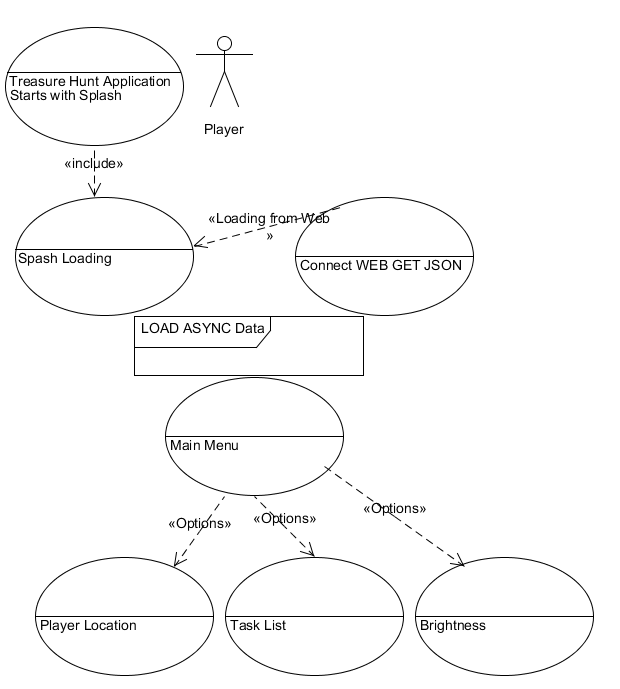
\includegraphics[scale=0.5]{dfd0}\\
\caption{DFD - 0 }
\label{the-label-for-cross-referencing}
\end{figure}
 % adds the Project Design
	\makeatletter
	\def\@makechapterhead#1{%
	  \vspace*{50\p@}%
	  {\parindent \z@ \centering\normalfont
	    \ifnum \c@secnumdepth >\m@ne
	      \if@mainmatter
	         \Large\bfseries \@chapapp\space \thechapter
 	        \par\nobreak
	        \vskip 20\p@
	      \fi
	    \fi
	    \interlinepenalty\@M
	     \Large \bfseries #1\par\nobreak
	
	    \vskip 40\p@
	  }}
	\def\@makeschapterhead#1{%
	  \vspace*{50\p@}%
	  {\parindent \z@ \centering 
	    \normalfont
	    \interlinepenalty\@M
	    \Large\bfseries  #1\par\nobreak
	    \vskip 40\p@
	  }}
	\makeatother
	\titlespacing*{\chapter}{0pt}{0pt}{12pt}

\chapter{Modules}


\section{Module Description}
The modules functionality has been defined below with the snippets code

\subsection{Splash Startup}

A splash screen is an image that appears while a game or program is loading. It may also be used to describe an introduction page on a website. Splash screens cover the entire screen or simply a rectangle near the center of the screen. The splash screens of operating systems and some applications that expect to be run full-screen usually cover the entire screen.

Splash screens are typically used by particularly large applications to notify the user that the program is in the process of loading. They provide feedback that a lengthy process is underway. Occasionally, a progress bar within the splash screen indicates the loading progress. A splash screen disappears when the application's main window appears.
Splash screens typically serve to enhance the look and feel of an application or web site, hence they are often visually appealing. They may also have animations, graphics, and sound.

The Java programming language has a specific class for creating splash screens,  that handles standard splash screen functions, e.g. display an image centered on screen then disappears when the first program window opens.
Type the Code and Few lines here



\subsection{Async Task }

AsyncTask enables proper and easy use of the UI thread. This class allows to perform background operations and publish results on the UI thread without having to manipulate threads and/or handlers.

AsyncTask is designed to be a helper class around Thread and Handler and does not constitute a generic threading framework. AsyncTasks should ideally be used for short operations (a few seconds at the most.) If you need to keep threads running for long periods of time, it is highly recommended you use the various APIs provided by the java.util.concurrent pacakge such as Executor, ThreadPoolExecutor and FutureTask.

An asynchronous task is defined by a computation that runs on a background thread and whose result is published on the UI thread. An asynchronous task is defined by 3 generic types, called Params, Progress and Result, and 4 steps, called onPreExecute, doInBackground, onProgressUpdate and onPostExecute.

\lstinputlisting{async.py}

\subsection{JSON parser}

JSON (JavaScript Object Notation) is a lightweight data-interchange format. It is easy for humans to read and write.

 It is easy for machines to parse and generate. It is based on a subset of the JavaScript Programming Language, Standard ECMA-262 3rd Edition - December 1999. JSON is a text format that is completely language independent but uses conventions that are familiar to programmers of the C-family of languages, including C, C++, C#, Java, JavaScript, Perl, Python, and many others. These properties make JSON an ideal data-interchange language.

JSON is built on two structures:

\begin{description}
 \item[$\bullet$ ]  A collection of name/value pairs. In various languages, this is realized as an object, record, struct, dictionary, hash  table, keyed list, or associative array.
 \item[$\bullet$ ]  An ordered list of values. In most languages, this is realized as an array, vector, list, or sequence.

These are universal data structures. Virtually all modern programming languages support them in one form or another. It makes sense that a data format that is interchangeable with programming languages also be based on these structures.



\lstinputlisting{json.txt}

\end{description}
\subsection{SQL Lite Helper}
A helper class to manage database creation and version management.You create a subclass implementing onCreate (SQLiteDatabase), onOpen (SQLiteDatabase), and this class takes care of opening the database if it exists, creating it if it does not, and upgrading it as necessary. Transactions are used to make sure the database is always in a sensible state.This class makes it easy for ContentProvider implementations to defer opening and upgrading the database until first use, to avoid blocking application startup with long-running database upgrades.Exposes methods to manage a SQLite database.SQLiteDatabase has methods to create, delete, execute SQL commands, and perform other common database management tasks.See the Notepad sample application in the SDK for an example of creating and managing a database.Database names must be unique within an application, not across all applications
\lstinputlisting{sqllitehelper.py}

\subsection{GPS Receiver}

Android gives your applications access to the location services supported by the device through classes in the android.location package. The central component of the location framework is the LocationManager system service, which provides APIs to determine location and bearing of the underlying device (if available).As with other system services, you do not instantiate a LocationManager directly. Rather, you request an instance from the system by calling LOCATION_SERVICE.


\lstinputlisting{gps.py}


\subsection{Google Maps API}
With the Google Maps Android API, you can add maps to your app that are based on Google Maps data. The API automatically handles access to Google Maps servers, data downloading, map display, and touch gestures on the map. You can also use API calls to add markers, polygons and overlays, and to change the user's view of a particular map area.

The key class in the Google Maps Android API is MapView. A MapView displays a map with data obtained from the Google Maps service. When the MapView has focus, it will capture keypresses and touch gestures to pan and zoom the map automatically,including handling network requests for additional maps tiles. It also provides all of the UI elements necessary for users to control the map. Your application can also use MapView class methods to control the map programmatically and draw a number of overlays on top of the map.

The Google Maps Android APIs are not included in the Android platform, but are available on any device with the Google Play Store running Android 2.2 or higher, through Google Play services.
To integrate Google Maps into your app, you need to install the Google Play services libraries for your Android SDK..
%\begin{figure} [ht]
%\centering
%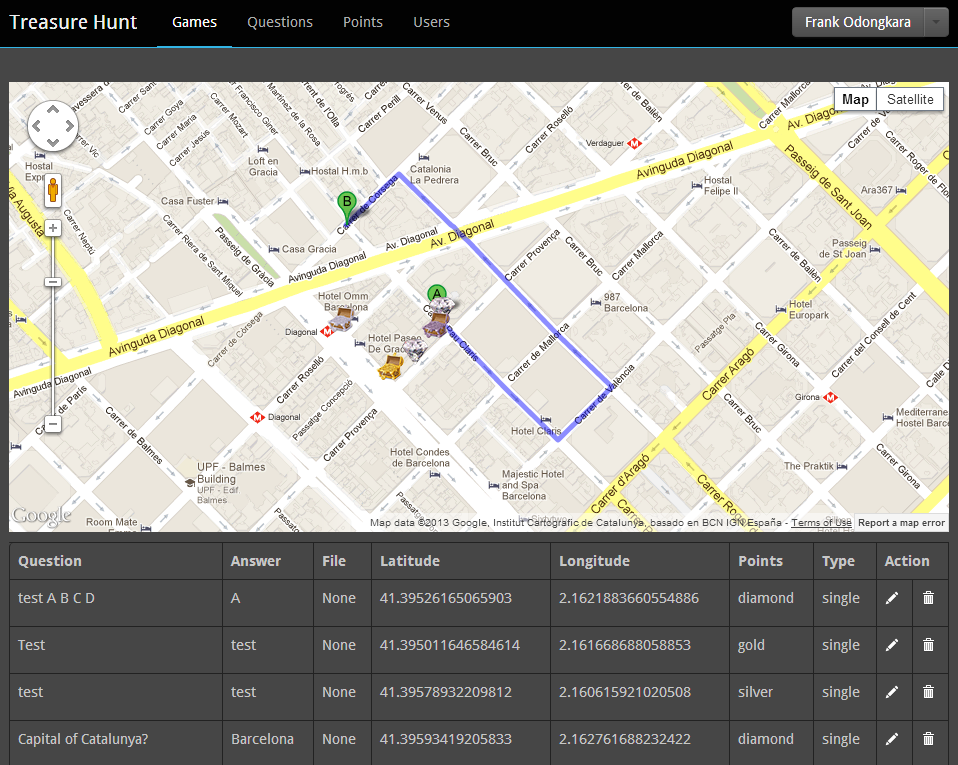
\includegraphics[scale=0.5]{images/maps}\\
%\caption{Custom Maps Designed }
%\label{Game Master Designs the Game with this Map}
%\end{figure}








 % adds the Project Design

\chapter{Implementation}


\section{\ignorespacesSource Code & Screen Shots}

\subsection{Splash Screen}

\begin{wrapfigure}{r}{0.3845\linewidth}
\centering
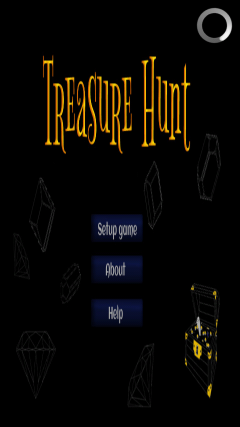
\includegraphics[scale=0.7]{snaps/splash}
\caption{Application Loading}
\label{fig:myfig}
\end{wrapfigure}
\textnormal{Splash Screen is a view that appears for sometimes (3 or 4 seconds).After dislaying splash screen that never comes second time in application until we restart Application.The purpose of a splash screen is to give the user an indication that your app is loading–not to create an extra delay before the user can load your app. People don’t like waiting, especially in a mobile environment.Using Thread,AsyncTask,Handler you can wait sometimes to load your app.The most desirable way to display splash screen is handler.you can do it easily.no need to create thread or async task in your activity.The handler have post Delayed (Runnable,long)  method.using this method you can wait some times to load app.Handler instance is associated with a single thread and that thread's message queue. When you create a new Handler, it is bound to the thread / message queue of the thread that is creating it -- from that point on, it will deliver messages and runnables to that message queue and execute them as they come out of the message queue.

}





%\lstinputlisting{java/splash.java}


\subsection{Location Marker}

\begin{wrapfigure}{r}{0.39\linewidth}
\centering
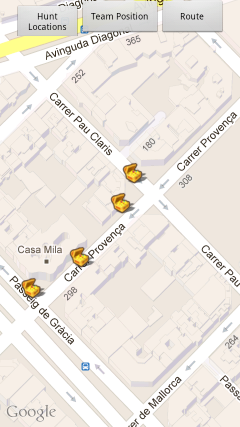
\includegraphics[scale=0.6]{snaps/location}
%\rule{0.9\linewidth}{0.75\linewidth}
\caption{Location Marker Activity}
\label{fig:myfig}
\end{wrapfigure}
\textnormal{
Location Marker is responsible  for plotting the real time location of all the user participating in the game. The functionality is when the player starts the application and registers it,the device starts sending the user co-ordinates to our webserver which is send back to other user using the JSON type in callback which uses the overlays on Android Maps to plot it.

In order to use the Android Maps you need to have maps and its API keys . The Treasure Hunt Icons are saved in the assets folder and the images are scaled for the device screen size and are in the PNG format.Using this Location Marker the user is not only able to see his locations but other locations where the other team are heading .

}

%\lstinputlisting{java/LocationMarker.java}

\subsection{Task List}

Treasure Hunting Game not only remains the concept of hunting treasures with maps but also integrates GPS function. With a designed route for treasure hunting, the students would not miss any places for treasures. During the process of game, students can participate in the activity and observe the environment in person and absorb the knowledge unconsciously. Meanwhile, students can learn how to apply GPS and the skills of reading maps to obtain the knowledge happily.Treasure Hunting Game not only remains the concept of hunting treasures with maps but also integrates GPS function. With a designed route for treasure hunting, the students would not miss any places for treasures. During the process of game, students can participate in the activity and observe the environment in person and absorb the knowledge unconsciously. Meanwhile, students can learn how to apply GPS and the skills of reading maps to obtain the knowledge happily.

\begin{equation*}
  \begin{CD}
    a @>>> b \\
    @VVV @AAA \\
    c @= d
  \end{CD}
  \qquad
  \begin{CD}
    x @>>\alpha> y \\
    @VV\kappa V @A\beta AA \\
    v @<\gamma<< w
  \end{CD}

\end{equation*}

%\lstinputlisting{java/TaskList.java}

\subsection{User Registration}

Treasure Hunting Game can only be played when the user has registered with the server and his device IMSI has been saved on the server,Once the user Installs the Application the user is asked to register the device and select team color , this is achieved using the registration class . A seperate XML layout has been developed for the Registration form . Once the data has been saved the entry is created in Shared Preferences and the application sends the data to webserver , the type of data is UTF-8 and in JSON format

\begin{align*}
\xymatrix@R=10pt{
    cRing \ar[r] & Sch \\
    A \ar@{}[u]|{\rotatebox{90}{$\in$}} \ar@{|->}[r] 
            & Spec(A) \ar@{}[u]|{\rotatebox{90}{$\in$}}
}
\end{align*}



\chapter{Snapshot}

\begin{figure}[h]
\begin{center}$
\begin{array}{cc}
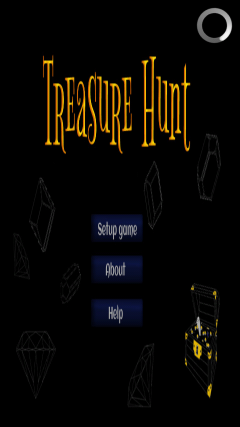
\includegraphics[width=2.5in]{snaps/splash} &
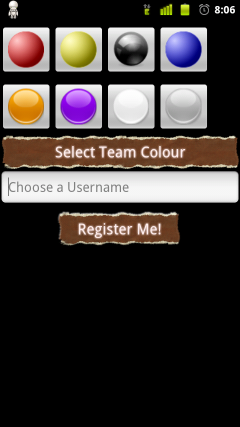
\includegraphics[width=2.5in]{snaps/user} &

\end{array}$
\end{center}
\caption{Spash Screen & Team Select}
\end{figure}

\begin{figure}[h]
\begin{center}$
\begin{array}{cc}
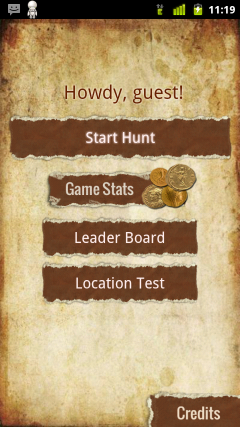
\includegraphics[width=2.5in]{snaps/3} &
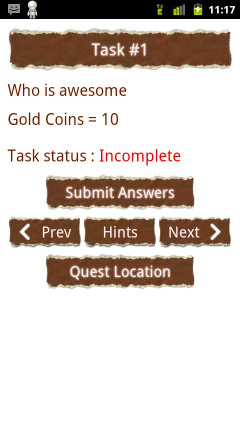
\includegraphics[width=2.5in]{snaps/4} 
\end{array}$
\end{center}
\caption{Main Menu & Task List}
\end{figure}

\begin{figure}[h]
\begin{center}$
\begin{array}{cc}
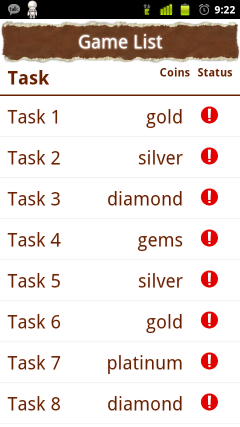
\includegraphics[width=2.5in]{snaps/5} &
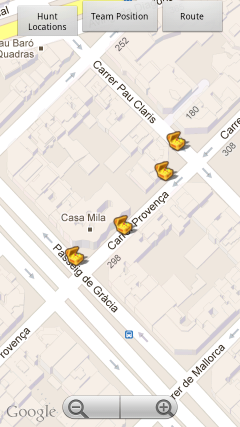
\includegraphics[width=2.5in]{snaps/6} 
\end{array}$
\end{center}
\caption{OverLays Map & Custom Location}
\end{figure}

\begin{figure}[h]
\begin{center}$
\begin{array}{cc}
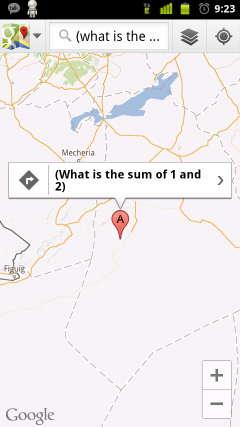
\includegraphics[width=2.5in]{snaps/7} &
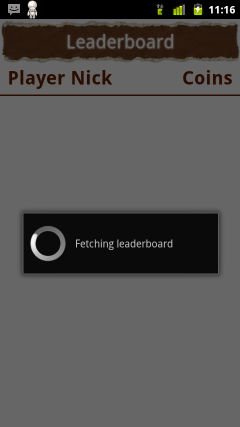
\includegraphics[width=2.5in]{snaps/8} 
\end{array}$
\end{center}
\caption{Async Loading using Simple Adapter}
\end{figure}

\begin{figure}[h]
\begin{center}$
\begin{array}{cc}
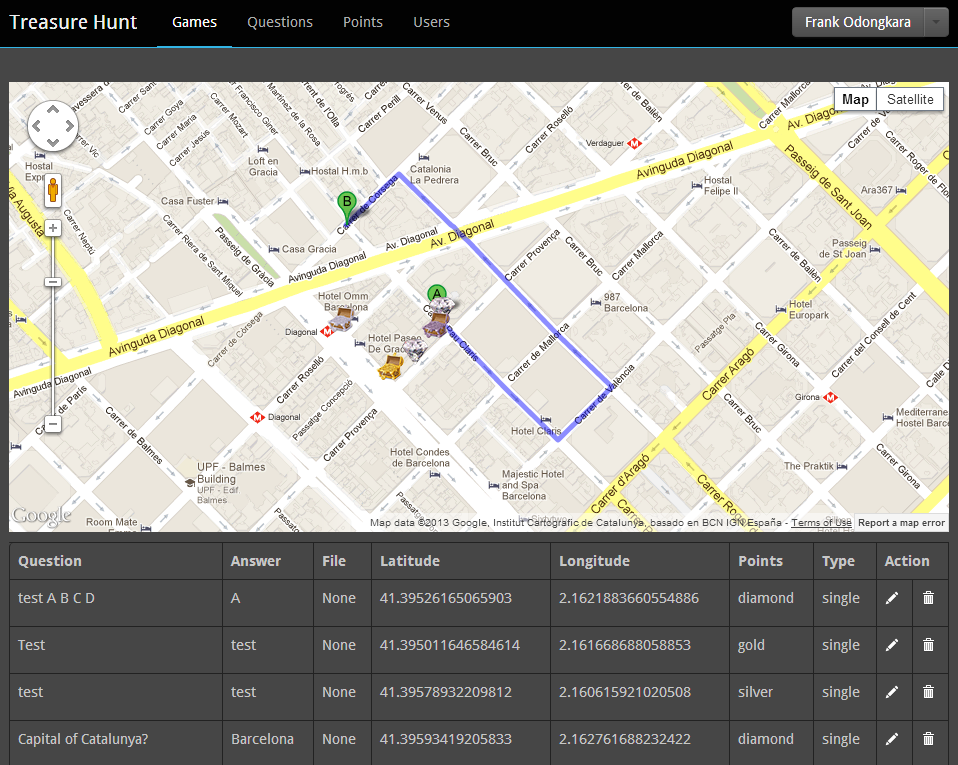
\includegraphics[width=2.5in]{images/maps} &
\end{array}$
\end{center}
\caption{Google Maps on Server }
\end{figure}





\chapter{Future Aspects}

Being build with the power of Cloud and Android this will have many uses , Its not long back when on April 1 2013 Google Released location where actual treasures were found by treasure hunters where other native people considered that as a April fools day Ha-ox. Implementing In Video on Google Customized Maps over Overlays and Custom route navigation with intelligent navigation is what will be released in the next release . The Application can be found on Google Play under the name of Treasure Hunt [Ankit APPS] \\

\chapter{Conclusion}

Treasure Hunting Game not only remains the concept of hunting treasures with maps but also integrates GPS function. With a designed route for treasure hunting, the students would not miss any places for treasures. During the process of game, students can participate in the activity and observe the environment in person and absorb the knowledge unconsciously. Meanwhile, students can learn how to apply GPS and the skills of reading maps to obtain the knowledge happily.








\end{adjustwidth} % adds the introduction page

\chapter{Scheduling}

\section{Executors}

Executor is a simple standardized interface for defining custom thread-like subsystems, including thread pools, asynchronous IO, and lightweight task frameworks. Depending on which concrete Executor class is being used, tasks may execute in a newly created thread, an existing task-execution thread, or the thread calling execute, and may execute sequentially or concurrently. ExecutorService provides a more complete asynchronous task execution framework. An ExecutorService manages queuing and scheduling of tasks, and allows controlled shutdown. The ScheduledExecutorService subinterface and associated interfaces add support for delayed and periodic task execution. ExecutorServices provide methods arranging asynchronous execution of any function expressed as Callable, the result-bearing analog of Runnable. A Future returns the results of a function, allows determination of whether execution has completed, and provides a means to cancel execution. A RunnableFuture is a Future that possesses a run method that upon execution, sets its results.Implementations. Classes ThreadPoolExecutor and ScheduledThreadPoolExecutor provide tunable, flexible thread pools. The Executors class provides factory methods for the most common kinds and configurations of Executors, as well as a few utility methods for using them. Other utilities based on Executors include the concrete class FutureTask providing a common extensible implementation of Futures, and ExecutorCompletionService, that assists in coordinating the processing of groups of asynchronous tasks.


\subsection{Queues}
The ConcurrentLinkedQueue class supplies an efficient scalable thread-safe non-blocking FIFO queue.
Five implementations in  support the extended Blocking Queue interface, that defines blocking versions of put and take: Linked Blocking Queue, Array Blocking Queue, Synchronous Queue, Priority Blocking Queue, and Delay Queue.The different classes cover the most common usage contexts for producer-consumer, messaging, parallel tasking, and related concurrent designs.The Blocking Deque interface extends BlockingQueue to support both FIFO and LIFO (stack-based) operations. Class Linked Blocking Deque provides an implementation.


\subsection{Timing}
The TimeUnit class provides multiple granularities (including nanoseconds) for specifying and controlling time-out based operations. Most classes in the package contain operations based on time-outs in addition to indefinite waits. In all cases that time-outs are used, the time-out specifies the minimum time that the method should wait before indicating that it timed-out. Implementations make a "best effort" to detect time-outs as soon as possible after they occur. However, an indefinite amount of time may elapse between a time-out being detected and a thread actually executing again after that time-out. All methods that accept timeout parameters treat values less than or equal to zero to mean not to wait at all. To wait "forever", you can use a value of Long.MAX_VALUE.


\subsection{Synchronizers}

Besides Queues, this package supplies Collection implementations designed for use in multithreaded contexts: ConcurrentHashMap, Concurrent Skip ListMap, ConcurrentSkipListSet, CopyOnWriteArrayList, and CopyOnWriteArraySet. When many threads are expected to access a given collection, a ConcurrentHashMap is normally preferable to a synchronized HashMap, and a ConcurrentSkipListMap is normally preferable to a synchronized TreeMap. A CopyOnWriteArrayList is preferable to a synchronized ArrayList when the expected number of reads and traversals greatly outnumber the number of updates to a list.The "Concurrent" prefix used with some classes in this package is a shorthand indicating several differences from similar "synchronized" classes. For example java.util.Hashtable and Collections.synchronizedMap(new HashMap()) are synchronized. But ConcurrentHashMap is "concurrent". A concurrent collection is thread-safe, but not governed by a single exclusion lock. In the particular case of ConcurrentHashMap, it safely permits any number of concurrent reads as well as a tunable number of concurrent writes. "Synchronized" classes can be useful when you need to prevent all access to a collection via a single lock, at the expense of poorer scalability. In other cases in which multiple threads are expected to access a common collection, "concurrent" versions are normally preferable. And unsynchronized collections are preferable when either collections are unshared, or are accessible only when holding other locks.Most concurrent Collection implementations (including most Queues) also differ from the usual java.util conventions in that their Iterators provide weakly consistent rather than fast-fail traversal. A weakly consistent iterator is thread-safe, but does not necessarily freeze the collection while iterating, so it may (or may not) reflect any updates since the iterator was created.

\section{Memory Consistency Properties}

 The synchronized and volatile constructs, as well as the Thread.start() and Thread.join() methods, can form happens-before relationships. In particular:
Each action in a thread happens-before every action in that thread that comes later in the program's order.An unlock (synchronized block or method exit) of a monitor happens-before every subsequent lock (synchronized block or method entry) of that same monitor. And because the happens-before relation is transitive, all actions of a thread prior to unlocking happen-before all actions subsequent to any thread locking that monitor.A write to a volatile field happens-before every subsequent read of that same field. Writes and reads of volatile fields have similar memory consistency effects as entering and exiting monitors, but do not entail mutual exclusion locking.A call to start on a thread happens-before any action in the started thread.All actions in a thread happen-before any other thread successfully returns from a join on that thread.The methods of all classes in java.util.concurrent and its subpackages extend these guarantees to higher-level synchronization. In particular:Actions in a thread prior to placing an object into any concurrent collection happen-before actions subsequent to the access or removal of that element from the collection in another thread.Actions in a thread prior to the submission of a Runnable to an Executor happen-before its execution begins. Similarly for Callables submitted to an ExecutorService.Actions taken by the asynchronous computation represented by a Future happen-before actions subsequent to the retrieval of the result via Future.get() in another thread.Actions prior to "releasing" synchronizer methods such as Lock.unlock, Semaphore.release, and CountDownLatch.countDown happen-before actions subsequent to a successful "acquiring" method such as Lock.lock, Semaphore.acquire, Condition.await, and CountDownLatch.await on the same synchronizer object in another thread.For each pair of threads that successfully exchange objects via an Exchanger, actions prior to the exchange() in each thread happen-before those subsequent to the corresponding exchange() in another thread.Actions prior to calling CyclicBarrier.await and Phaser.awaitAdvance (as well as its variants) happen-before actions performed by the barrier action, and actions performed by the barrier action happen-before actions subsequent to a successful return from the corresponding await in other threads.

XXXXXXX
\end{adjustwidth} % adds the Scheduling and Planning page
\chapter{Conclusion }

Treasure Hunting Game not only remains the concept of hunting treasures with maps but also integrates GPS function. With a designed route for treasure hunting, the students would not miss any places for treasures. During the process of game, students can participate in the activity and observe the environment in person and absorb the knowledge unconsciously. Meanwhile, students can learn how to apply GPS and the skills of reading maps to obtain the knowledge happily.


 % adds the Scheduling and Planning page
%\chapter{Future Scope}


\section{Future Scope}





 % adds the Scheduling and Planning page

\begin{thebibliography}{99}
\addcontentsline{toc}{chapter}{\bibname}
\lhead{}\markboth{\bibname}{}

% \bibitem{TEXT} is how you refer to your reference in your report. keep that very short
% \emph{Paper Name} is just to highligh the paper name by making it italic, not required but looks nice

%Example
\bibitem{The Joy of Geocaching}\emph{The Joy of Geocaching};  by Paul and Dana Gilline, ISBN 1-88495-699-8)
\bibitem{The Essential Guide to Geocaching}\emph{The Essential Guide to Geocaching};  DK Publishing (ISBN 978-0-7566-3717-0)
\bibitem{The Complete Idiot's Guide }\emph{The Complete Idiot's Guide};  Jeannette Cézanne (ISBN 978-1-60166-004-6)
\bibitem{The Geocaching Handbook}\emph{The Geocaching Handbook}; Joel McNamara (ISBN 978-0-7645-7571-6)
\bibitem{Sharing GPS }\emph{Sharing GPS };  by Norman Lukeman, ISBN 1-84533-302-1)
\bibitem{PMS System }\emph{PMS System };  by Bhavin Mehta IJSER , ISBN 1-92534-402-4)


%And how you would refer to the paper in the text - example
%Your text in other tex files \cite{short_paper_name} contd explaining

%If you have to display links, do it via  adding \\ (newline) otherwise it goes off the margins. Don't know how to fix this yet
%\bibitem{short_link_name}Link Name \\ \url{http://url link here}
%\url{The-human-element-the-weakest}



\end{thebibliography} % adds the References page

\newpage
\appendix
\section{\\Title of Appendix A} \label{App:AppendixA}
% the \\ insures the section title is centered below the phrase: AppendixA

Text of Appendix A is Here

\newpage
\section{\\Title of Appendix B} \label{App:AppendixB}}
% the \\ insures the section title is centered below the phrase: Appendix B

Text of Appendix B is Here

\newpage
\begin{thebibliography}{10}



\end{thebibliography}

\end{document}
